
\newcommand{\FigOverview}{
\begin{figure*}[t]
    \centering
    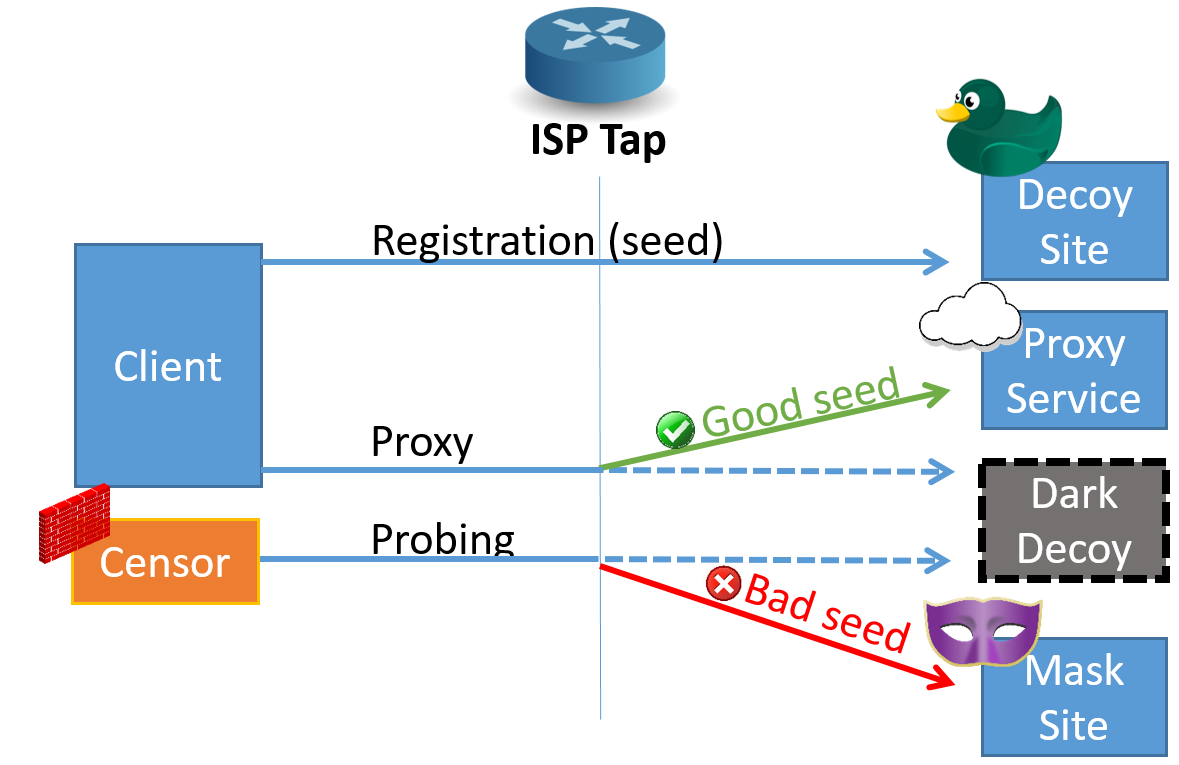
\includegraphics[width=0.60\linewidth,clip]{figures/dark-decoy-overview.png}
    \caption{\textbf{Dark Decoy Overview}\,---\, %
    }
    \label{fig:overview}
\end{figure*}
}

\newcommand{\FigHighLevel}{
\begin{figure}[t]
    \centering
    \vspace{-0.5in}
    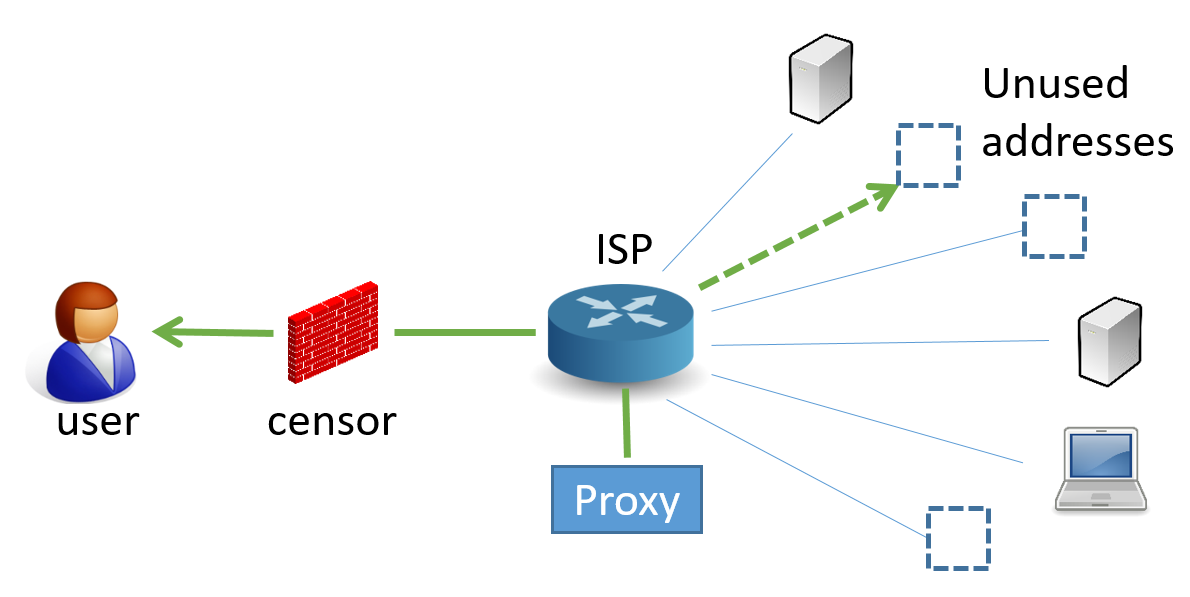
\includegraphics[width=\linewidth,clip]{figures/high-level.png}
    \caption{\textbf{Overview}---%
      When deployed at an ISP, \scheme observes a mirror of inbound and outbound traffic.
      Users request service by embedding a steganographic registration message in a TLS handshake with any reachable site at the ISP\@. Then, the client connects to a random unused (``dark'')
      address in the ISP's AS, and \scheme communicates with the client as if it were a proxy at that address.
    }
    \label{fig:overview}
\end{figure}
}


\newcommand{\yes}{\CIRCLE}
\newcommand{\no}{\Circle}
\newcommand{\maybe}{\LEFTcircle}

\newcommand{\TabCompare}{
\begin{table*}[ht]
    \centering
    \begin{tabular}{l|cccccccc}
            % Multiflow? Waterfall?
            & \rot{Telex~\cite{telex11}} &
            \rot{Cirripede~\cite{cirripede11}} &
            \rot{Decoy Routing~\cite{curveball11}} &
            \rot{TapDance~\cite{tapdance14}} & \rot{Rebound~\cite{rebound15}} & \rot{Slitheen~\cite{slitheen16}} & \rot{Waterfall~\cite{waterfall}} & \rot{\textbf{Dark Decoys}} \\
            \hline
                                      %Telex Cirr  DR     TD      RB    Slth   Water  DD
            No inline blocking        & \no & \no  & \no & \yes  & \no  & \no  & \no  & \yes \\
            Handles asym. routing     & \no & \yes & \no  & \yes & \yes & \no  & \yes & \yes \\
            Currently deployed        & \no & \no  & \no  & \yes & \no  & \no  & \no  & \no \\
            Replay attack resistant   &\yes & \yes & \yes & \no  & \yes & \yes & \yes & \yes \\
            Traffic analysis resitant &\no  & \no  & \no  & \no  &\maybe& \yes &\maybe& \no \\
            Uses unused addresses     & \no & \no  & \no  & \no  & \no  & \no  & \no  & \yes \\
    \end{tabular}
    \caption{\textbf{Comparing Refraction Networking schemes}\,---\,}
    \label{tab:compare}
\end{table*}
}



\newcommand{\FigImplementation}{
\begin{figure}[ht]
    \centering
    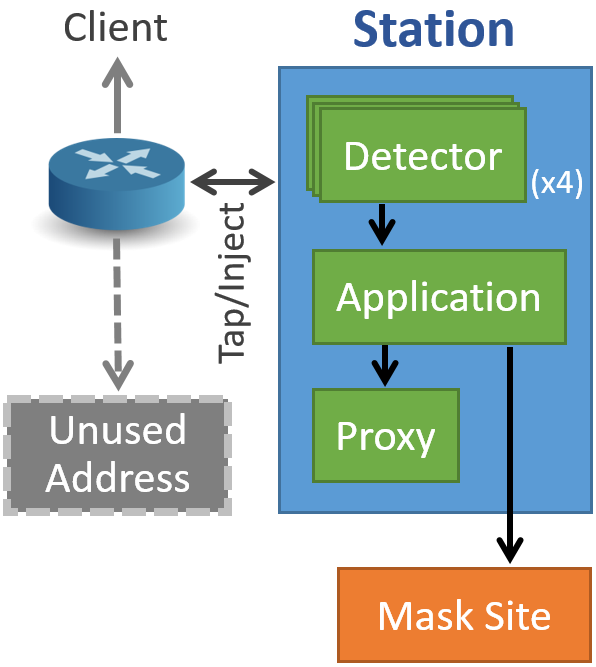
\includegraphics[width=0.7\linewidth,clip]{figures/implementation.png}
    \caption{\textbf{Station Architecture}\,---\, %
    }
    \label{fig:implementation}
\end{figure}
}

\newcommand{\FigEvolution}{
\begin{figure}
  \centering
  \begin{subfigure}{\columnwidth}
    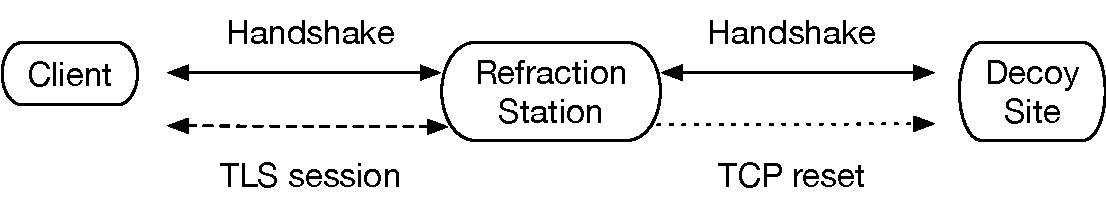
\includegraphics[width=\columnwidth]{figures/refraction-v1}
    \vspace{-3pt}
    
    \caption{\textbf{First generation systems} for Refraction Networking, such as Telex and Cirripede, operated as inline network elements, with the ability to observe traffic and block specific flows. ISPs worried that if the inline element failed, it could bring down the network.\looseness=-1}
    \label{fig:refraction-v1}
  \end{subfigure}
  \vspace{16pt}
  
  \begin{subfigure}{\columnwidth}
    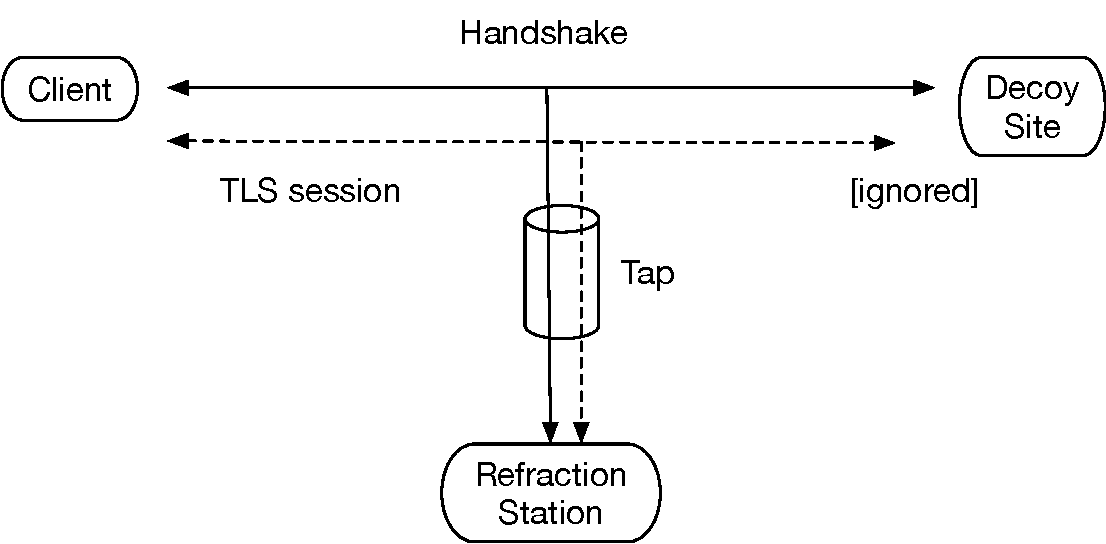
\includegraphics[width=\columnwidth]{figures/tapdance}
    \vspace{-3pt}
    
    \caption{\textbf{TapDance} is a second-generation Refraction Network scheme that operates without flow blocking, needing only to passively observe traffic and inject packets. TapDance has recently been deployed at a mid-size ISP, but the techniques used to silence the decoy site and participate in the client--decoy TCP connection mid-stream add significant complexity, performance bottlenecks, and detection risk.}
    \label{fig:tapdance}
  \end{subfigure}
  \vspace{16pt}
  
  \begin{subfigure}{\columnwidth}
    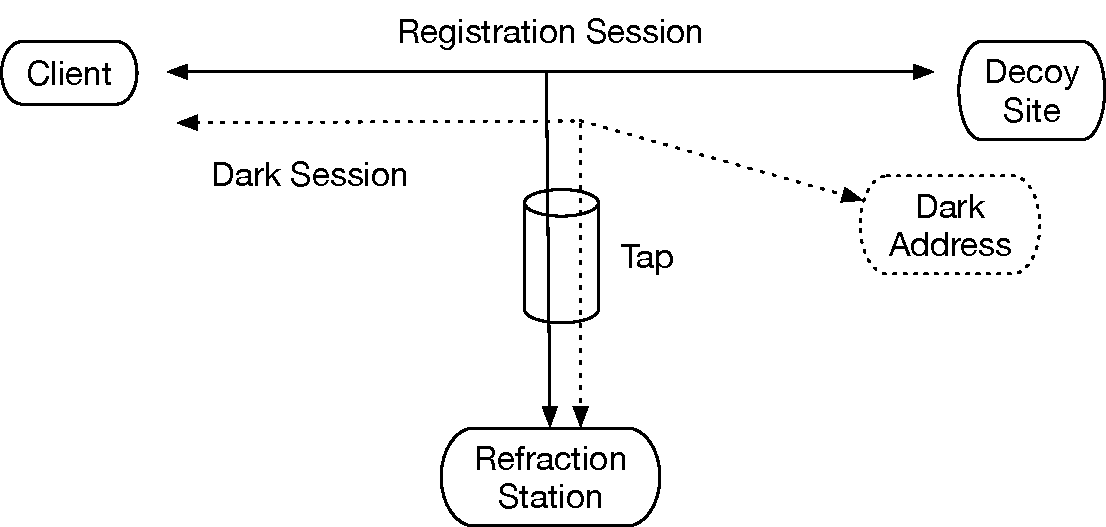
\includegraphics[width=\columnwidth]{figures/dark-decoys}
    \vspace{-3pt}
    
    \caption{\textbf{\scheme}, our third-generation Refraction Networking design, overcomes these limitations.  It uses two sessions. First, the client connects to a decoy site and embeds a steganographic registration message, which the station receives using only a passive tap.  Second, the client connects to a ``dark address'' where there is no running server, and the station proxies the connection in its entirety.}
    \label{fig:dark-decoys}
  \end{subfigure}

  \vspace{12pt}
  \caption{\textbf{Evolution of Refraction Networking Approaches}}
\end{figure}
}
